\documentclass[12pt]{article}
\usepackage[margin=1in]{geometry}

% The preceding line only needs to identify funding in the first footnote. If that is unnecessary, please comment on it.
\usepackage{float}
\usepackage[table]{xcolor}
\usepackage{cite}
\usepackage{subcaption}
\usepackage{multirow}
\usepackage{graphicx}
\usepackage{amsmath,amssymb,amsfonts}
\usepackage{algorithmic}
\usepackage{graphicx}
\usepackage{textcomp}
\usepackage{xcolor}
\usepackage{multirow}
\usepackage{setspace}
\usepackage{tabularx}
\usepackage{url}
\usepackage{tabularray}
\usepackage{makecell}
\usepackage{placeins}
\usepackage{comment}
\usepackage{verbatim}
\usepackage{rotating}
\usepackage{chngpage}
\renewcommand{\cellalign}{cl}

\usepackage{booktabs, multirow} % for borders and merged ranges
\usepackage{soul}% for underlines
\usepackage[table]{xcolor} % for cell colors
\usepackage{changepage,threeparttable} % for wide tables

\def\BibTeX{{\rm B\kern-.05em{\sc i\kern-.025em b}\kern-.08em
    T\kern-.1667em\lower.7ex\hbox{E}\kern-.125emX}}
    
    
    \newcommand*{\affaddr}[1]{#1} % No op here. Customize it for different styles.
\newcommand*{\affmark}[1][*]{\textsuperscript{#1}}
\newcommand*{\email}[1]{\textit{#1}}
    
\begin{document}
\begin{center}
\Large
\thispagestyle{empty}

\textbf{Deception Detection Models from Speech}\\
\vspace{0.1in}
\large
\text{A Project Report}\\
\vspace{2in}

\text{Presented to}\\
\text{The Faculty of the Department of Computer Science}\\
\text{San Jose State University}\\

\vspace{1in}

\text{In Partial Fulfillment}\\
\text{of the Requirements for the Degree of}\\
\text{Master of Science}\\

\vspace{1in}

\text{By}\\
\text{Tien Nguyen}\\
\text{Spring 2024}\\

\end{center}

\title{}
\newpage
\thispagestyle{empty}
\begin{center}
\Large
\text{The Designated Project Committee Approves the Project Titled}\\
\vspace{0.1in}
\Large
\text{Deception Detection Models from Speech}\\
\vspace{0.5in}
\text{by}\\
\vspace{0.1in}
\text{Tien Nguyen}\\
\vspace{1.5in}
\Large
\text{APPROVED FOR THE DEPARTMENT OF COMPUTER SCIENCE} \\
\vspace{0.1in}
\text{SAN JOSÉ STATE UNIVERSITY} \\
\vspace{0.1in}
\text{Spring 2024}\\
\vspace{1.5in}
\Large
\begin{tabular}{lcl}
Prof. Faranak Abri & \hspace{1cm} & Department of Computer Science \\
Prof. Nada Attar & \hspace{1cm} & Department of Computer Science \\
Prof. Fabio Di Troia & \hspace{1cm} & Department of Computer Science \\
\end{tabular}
 

\end{center}
\newpage

\pagenumbering{roman}
%\linespread{1.5} 

\doublespacing
\section*{Abstract}
\bigskip
Recently, researchers have shown an increased interest in automatically detecting deceptive actions. The attention given to this area can be attributed to the many potential applications of deception detection, especially in the field of criminology. To contribute to the deception detection research, this project investigates textual and audio data extracted from spoken and written words. We evaluated and compared the traditional linguistic models with advanced Large Language Models (LLMs) while using Natural Language Processing (NLP) techniques. Additionally, various feature selection techniques were applied to assess the importance of linguistic features. We conducted extensive experiments to evaluate the effectiveness of both conventional and deep NLP models on textual data. In addition, the deep models were also applied to audio data. Findings suggest that the best-performing models for each data type are the Bidirectional Long Short Term Memory for textual data and the ResNet50 for audio data. These models were then combined to create a late fusion model that outperforms other text and audio models from previous research using the measures of accuracy and F1 score for comparison. This late fusion model achieved an impressive score with an accuracy of 90.9$\%$ and an F1 score of 91.07$\%$.\\

\noindent \textbf{Keywords:} Deception Detection, Natural Language Processing (NLP), Large Language Models (LLM), Audio Data Processing, Multimodal
\newpage
%-------------------------------------------------------------------------------------------------
\section*{Acknowledgements}
I would like to express my sincere gratitude to my advisor, Professor Faranak Abri, for her invaluable guidance and support throughout this project. Her insights and feedback have helped me navigate challenges and achieve my goals. Thank you for your mentorship and encouragement.\\
  
\noindent
I would like to extend my gratitude to all members of my defense committee, Professor Nada Attar and Professor Fabio Di Troia.\\

\noindent  
I would like to extend my heartfelt thanks to my family and friends for their unwavering support and encouragement throughout my academic journey and in all aspects of my life.

\bigskip

\newpage
\tableofcontents
\newpage
\bigskip
\listoffigures
\listoftables


\newpage
\vspace{-0.1in}
\pagenumbering{arabic}
\section{Introduction}
\label{sec:intro}
People have always used deception to manipulate or take advantage of others' trust for their own benefit. Lying can hurt friendships or family bonds. It can be used to scam innocent people out of their money or mislead a criminal investigation. These actions can lead to serious consequences, such as innocent people being wrongly convicted or losing money. With that motivation in mind, finding out when someone is not telling the truth could help avoid damage in both personal and work relationships. 
Moreover, identifying when people are not telling the truth is crucial for finding out what happened and supporting fair treatment in court cases. As a result, the ability to detect dishonest statements is a solution to the dilemma that our society faces every day. 
  
The power to know for certain whether a person is telling the truth or lying is a long-sought-after ability. 
One example of this is a Polygraph test which has long been considered the method for detecting lies. However, these tests are not nearly accurate enough. They are prone to errors and biases arising from both the equipment used and human misinterpretation. A better alternative, multi-modal lie detection techniques, can be employed to address the issues of inaccuracy associated with polygraph tests. Specifically, analyzing speech data can provide a wealth of information to identify instances of deceitfulness. One potential approach is to examine characteristics in speech, such as changes in pitch, speaking rate, and intensity, which can occur when someone is untruthful. Another potential approach involves analyzing features in speech, such as word choice and sentence structure, which can also serve as indicators of deception. Additionally, considering nonverbal cues, like expressions, body language, and eye movements, is another feasible approach for detecting deceptive behavior.

The recent advancement in machine learning and deep learning algorithms enables the creation of classification schemes trained on these multi-modal features to accurately classify people's truthfulness in a given case or scenario. The use of machine learning in lie detection has gained significant attention in recent years, with many researchers achieving promising results in accurately detecting deception from speech by combining these features and using machine learning algorithms~\cite{talaat2023explainable},~\cite{aslan2023lstmncp}.

  
The goal of this project is to create a model using textual and audio data to detect deceptive contexts.
By developing more reliable and accurate lie detection models, we could provide reliable support to individuals from the harmful consequences of deception and ensure the integrity of legal proceedings. The key contributions of this paper are as follows:

\begin{enumerate}
\item Development of a Minimalistic Feature Set: We identified and utilized relevant linguistic features for deception detection. This avoids irrelevant data, leading to more efficient and accurate detection.

\item Innovative Use of Feature Selection Techniques: Various feature selection methods in this paper, including the stepwise approach and the Overlapping Coefficient (OVL) method, have enhanced the understanding of feature importance in deception detection.

\item Comparative Analysis of Conventional and LLM-Based Models: This study compares traditional NLP models and advanced LLMs on textual data.

\item Development of Audio-Based Deception Detection Model: We constructed deep models using audio data.

\item Implementation of a Late Fusion Technique: The outputs of the textual and audio models are combined using a late fusion approach. 

\item  Experimentation on Real-Life dataset: The models are applied to the Real-Life Trial dataset to ensure that our findings are based on practical, real-world scenarios.

\end{enumerate}

The structure of this paper is as follows: Section II reviews existing research in the deception detection field. Section III outlines our methodology. Section IV outlines the experimental setup, giving specifics on the dataset, preprocessing, feature selection, and evaluation metrics. Section V discusses the setup of the detection model. Section VI presents the results. Section VII discusses these results, providing insights into various approaches' effectiveness and alignment with existing literature. Lastly, section VIII concludes the paper and suggests future work.
 



%--------------------------------------------------------------------------------------------------
\section{Related Work}
This section will review datasets and models used and implemented in the previous deception detection research.
\subsection{Dataset}
In the process of training models that are capable of detecting deception, a variety of datasets are utilized. These datasets are typically sourced from different contexts and scenarios, providing a wide range of data for the models to learn from. There are three main categories each dataset can fall into. These categories focus on the source of the data. One category is any data collected from real-life situations where deception is common, such as legal proceedings. Data can also be generated artificially by prompting people with questions designed to force deception. Finally, data can also be collected while playing games, where deception can also commonly and naturally occur.

The first category of data was collected and derived from various real-life situations. This type of dataset provides authentic examples of deception and truth-telling.  Instead of staged setups, these datasets can provide more realistic scenarios for lie detection. Several researchers [~\cite{bareeda2021lie},~\cite{hsiao2022attention},~\cite{csen2020multimodal},~\cite{sehrawat2023deception}] have utilized data that was collected from actual court trials. One particular dataset includes 121 videos that are divided into 61 clips that showcase deceptive behavior and 60 clips that feature truthful interactions. The individuals featured in these videos, who are either defendants or witnesses, range in age from 16 to 60. On average, the videos are approximately 28 seconds long, and the transcripts of these videos have an average of around 66 words, amounting to a total of over 8,000 words of speech data. Another notable dataset is used by Kopev et al.~\cite{kopev2019detecting}. This dataset is a real-world political debate dataset. This dataset offers a wider range of realistic situations for lie detection, including claims labeled as true, half-true, or false. This dataset consists of 94 training claims and 192 test claims, providing substantial data for the models to learn from.

Another dataset type was generated by prompting actors with questions designed to generate both deceptive and truthful responses. In a study by Wawer et al.,~\cite{sarzynska2023truth}, 400 participants were invited to create four statements on a given topic: two of these statements were to be delivered orally, while the other two were to be written. This method resulted in 1,600 statements, 1,498 of which were selected for the final analysis. Mendels et al.~\cite{mendels2017hybrid} used the CXD corpus, which comprises deceptive and non-deceptive speech from native English and Mandarin speakers, all communicating in English. It includes 170 conversations involving 340 participants. This data was gathered using a fake resume setup where subjects alternated between interviewer and interviewee roles, answering 24 biographical questions. Participants had financial incentives to both lie convincingly and accurately detect lies. During the interviews, the interviewees labeled each response as true or false. 
  

Data sets were also collected from playing games. Tao et al.~\cite{tao2019speech} used the IDIAP WOLF dataset developed by the Swiss IDIAP Research Institute. This study collected vocal signals from the "werewolf killing" game involving 12 participants, four of whom play werewolves aiming to create confusion through deception. The rest play honest characters. The werewolves are supposed to lie, while the other players are supposed to guess who the werewolves are. Similarly, Fu et al.~\cite{fu2023semi} created the H-Wolf corpus, a self-built dataset constructed from the Idiap Wolf and Killer datasets. They gathered approximately 70 hours of video from the "Werewolves of Miller’s Hollow" competitions available online, selecting clips that contained truthful and deceptive interactions based on the players' ID cards and the rules of each game.

\subsection{Conventional Models}
This section will introduce some of the conventional models used in previous work. Researchers have explored a variety of methodologies, ranging from traditional statistical models to advanced machine-learning techniques. Wawer et al.~\cite{sarzynska2023truth} implemented a Support Vector Machine (SVM) and XGBoost with 20-fold cross-validation. Their best model, SVM, gave an accuracy of 58.9 $\%$. 
  
Bareeda et al.~\cite{bareeda2021lie} built SVM-based classifiers using Gaussian and polynomial kernels. Based on experiments, they found that using either polynomial or Gaussian kernels resulted in an overall classification accuracy of 81$\%$ and 78$\%$ for the lie and truth classes, respectively. 
  
Tao et al.~\cite{tao2019speech} extracted different acoustic features to detect deception using SVM as the classifier. Before building the model, the extracted features were normalized. The experimental results showed that SVM could effectively detect deception with a recognition accuracy of over 80$\%$.
  
Chebbi et al.~\cite{chebbi2021deception} created K Nearest Neighbour (KNN) models for each modality separately using feature selection techniques to select the most relevant features. They combined the modalities using a decision-level fusion approach based on belief theory. The approach was tested using the Real-Life trial dataset ~\cite{csen2020multimodal}. The deception detection accuracy rate reached 97$\%$ using only 19 combined features.
  
Sen et al.~\cite{csen2020multimodal} collected videos from the actual trial and built models that used verbal, acoustic, and visual modalities to detect deception. Initially, they performed experiments with each set of features separately using SVM, Randon Forest (RF), and Neural Network (NN) classifiers. Then, they tried various combinations of features using early fusion and late fusion. The best accuracy (84.18\%) was achieved through late fusion, combining visual and acoustic features using the NN classifier. 
  
Venkatesh et al.~\cite{venkatesh2019robust} introduced a novel deception detection approach that utilized multiple data types, including audio, text, and non-verbal features. The method combined the results from each of these features using majority voting. Specifically, the audio component was based on Cepstral Coefficients (CC) and Spectral Regression Kernel Discriminant Analysis (SRKDA), the text model used bag-of-n-gram features and a linear SVM classifier, and the non-verbal component employed the AdaBoost classifier. The results showed that the proposed method outperformed both existing state-of-the-art techniques and human performance, achieving a deception detection accuracy of 97$\%$ on the entire dataset during 25-cross-fold validations.

\subsection{Deep Models}
Deep models have significantly impacted deception detection, bringing about a level of complexity that can detect minor details in data. In this section, we will look at previous work using deep models. Sehrawat et al.~\cite{sehrawat2023deception} proposed a model that combined Long-Short Term Memory (LSTM), Bidirectional LSTM networks (BiLSTM), Convolutional Neural Network (CNN), and ResNet50 to detect deception. They first extracted text, audio, and video features from the Real Life Court Trial dataset. To process audio data, they transformed it into Mel Spectrograms to create a visual representation that captured key audio characteristics. ResNet50 was then used to analyze these Mel Spectrograms. The proposed model, which utilized features from both audio and text, achieved an accuracy of 80$\%$. 
  
Unlike Sehrawat et al.~\cite{sehrawat2023deception}, who used an existing dataset, Marcolla et al.~\cite{marcolla2020novel} created their own dataset by interviewing subjects to capture the subject's answers, labeled as either lying or truthful. To get the audio features, the researchers used Librosa library functions to extract the Mel-Frequency Cepstral Coefficients (MFCC) characteristics. Then, the features were normalized through padding to match the length of the longest sequence, ensuring uniformity for neural network processing. Their LSTM neural network model resulted in an overall classification accuracy of 72.5$\%$. 
Hsiao and Sun~\cite{hsiao2022attention} also used MFCC for their audio feature. But instead of normalizing MFCC features to match the longest sequence, they calculated average MFCC values per second. This method reduced MFCC length, which helped train their BiLSTM model more effectively. They also extracted features from text and transcript. Lastly, they proposed an ensemble model that combined outputs from the audio, visual, and transcription models using BiLSTM. Their ensemble model achieved 96$\%$ accuracy when used on the Real Life Court Trial dataset. 
  
Antolín and Montero~\cite{gallardo2021detecting} developed an automatic deception detection model from gaze and speech features using attention LSTM. Feature extraction from gaze data involved selecting channels from the Gazepoint GP3 Eye Tracker for fixations, saccades, and pupil size, which are known indicators of deceptive behavior. For speech, features were derived from log-Mel Spectrograms using Python’s package LibROSA. The researchers trained their models on the Bag-of-Lies dataset and achieved an accuracy of  70.5$\%$.

Zhang et al.~\cite{zhang2022fine} created a Graph-based Cross-modal Fusion Model (GCFM) along with a Cross-modal Attention Mechanism to detect deception in the Real-Life Trial dataset ~\cite{csen2020multimodal}. They extracted visual, textual, and audio features by using a pre-trained ResNet50 and LSTM neural network with attention mechanisms. The proposed GCFM method achieved an accuracy of 88.14$\%$ as well as an F1-score of 78.50$\%$. Additionally, using association learning increased the accuracy by 1.87$\%$ while the cross-modal attention mechanism improved the accuracy by 2.44$\%$.
%\FloatBarrier
\begin{singlespace}
\begin{adjustwidth}{-2.5 cm}{-2 cm}\centering
\begin{threeparttable}[H]
\scriptsize
\begin{tabular}{l l l l l l l }
\hline
%\multicolumn{9}{|c|}{Exhaustive Search Results for the Best A/V Prediction} \\ \hline
{\bf Ref.} &
{\bf Dataset} &
{\bf Features} &
{\bf Modality} &
\makecell{\bf Classification\\ \bf Method}&
{\bf Metrics} &
{\bf Scores} \\ \hline
  
\cite{sarzynska2023truth}
& \makecell{ nearly 1,500 \\ true and false \\ statements}
& 43 features
& \makecell{transcription,\\ written}
& SVM
& Accuracy
& 58.9$\%$\\ \hline

\cite{mendels2017hybrid}
& \makecell{Columbia \\ X-Cultural \\ Deception}
& \makecell{ 
Ngrams, Acoustic-prosodic including\\ pitch, intensity, duration, voice\\ quality (jitter, shimmer, and\\ harmonics-to-noise ratio), spectral\\ harmonicity, and psychoacoustic \\spectral sharpness, MFCCs}
& \makecell{audio,\\ transcription}
& \makecell{Hybrid:\\ LSTM + DNN}
& \makecell{Precision\\ Recall \\ F1} 
& \makecell{67.32$\%$ \\ 60.80$\%$ \\ 63.90$\%$}    \\ \hline

\cite{kopev2019detecting} 
& Political debates 
& \makecell{LIWC, TF.IDF, i-vector, speaker \\ psychoacoustic spectral sharpness,\\ voice quality, energy, spectral, and \\ other low-level descriptors} 
& \makecell{audio,\\ transcription}
& \makecell{Logistic Regression,\\  multi-input\\ feed-forward \\ neural network} 
& \makecell{Accuracy \\ MAE \\ MMA \\ MA F1 \\ MAR} 
& \makecell{67 \\ 69$\%$  \\51.04$\%$  \\45.07$\%$  \\47.25$\%$ } \\ \hline

\cite{bareeda2021lie} 
&  \makecell{ Real-life trial} 
& \makecell{MFCC and mean of MFCC of all \\frames}
& audio 
& \makecell{ SVM using\\ polynomial kernel}  
& Accuracy   
& 81$\%$    \\ \hline

~\cite{fu2023semi} 
&  \makecell{ H Wolf } 
&  \makecell{acoustic statistics and time-\\frequency features}  
& \makecell{ audio } 
& \makecell{Hybrid\\ semi-supervised \\Neural Network}
& \makecell{Accuracy}   
& \makecell{68.62$\%$ }     \\ \hline
\cite{tao2019speech} 
& IDIAP WOLF 
& \makecell{fundamental frequency, Short-term\\ energy, Zero-crossing rate, MFCC,\\ other features} 
& video 
& SVM   
& Accuracy  
& 82.47$\%$   \\ \hline
  
\cite{hsiao2022attention} 
& Real-life trial 
&  136-dimension vectors 
& \makecell{visual, audio, \\transcription }& \makecell{ BiLSTM,\\ Ensemble\\ model (voting)}
& Accuracy
& 96$\%$    \\ \hline

\cite{csen2020multimodal}
& Real-life trial
& \makecell{ Unigrams, LIWC, Facial Displays,\\ Hand Gestures, Facial Action\\ Units (FACS), Pitch, Silence and \\Speech Histograms}
& \makecell{visual, audio,\\ transcription}
& NN
& Accuracy  
& 84.18$\%$    \\ \hline

\cite{venkatesh2019robust}
& Real-life trial
&  \makecell{ Ngrams, Audio subsystem: MFCCs, \\Log-Energy of MFCC, and CC, \\ Micro-expressions} 
& \makecell{visual, audio, \\transcription }
& \makecell{ SRKDA (audio) +\\ SVM (text) +\\AdaBoost\\(micro-expression)} 
& Accuracy   
& 97$\%$    \\ \hline

\cite{hu2019detecting}
&  \makecell{ Blind tasting \\ game}
&  \makecell{ LIWC, binary and numeric features \\capturing hedging linguistic and\\ syntactical distinctiveness, Acoustic-\\prosodic including intensity mean \\ and max, pitch mean and max, 3 \\ voice quality features (shimmer, jitter,\\ noise-to-harmonics ratio),\\ and speaking quality, MFCCs}
& \makecell{visual, audio, \\transcription }
& \makecell{ MLP + \\ BiLSTM +\\ Multi-task}
& F1
& 71.51$\%$    \\ \hline

\cite{chebbi2021deception}
&  \makecell{ Real-life trial}
&  \makecell{ pitch-based features, 21 Text-based\\ features: 
 the use of passive voice, \\ negative emotion words, deny words,\\ hasYes, laughing, crying, as well as\\ speech errors, etc.
}
& \makecell{visual, audio, \\transcription }
& \makecell{Hybrid: KNN}
& Accuracy
& 97$\%$    \\ \hline
  
\cite{zhang2022fine}
&  \makecell{ Real-life trial}
&  \makecell{21 pitch-based and spectral features, \\ BiLSTM text features, ResNet video\\ features }
& \makecell{visual, audio, \\transcription }
& \makecell{ GCFM + \\ early fusion \\(cross model attention)}
& \makecell{Accuracy \\ F1}
& \makecell{88.14$\%$ \\ 78.5$\%$}     \\ \hline

~\cite{sehrawat2023deception} 
&  \makecell{ Real-life trial} 
&  \makecell{Mel Spectrograms features, \\ word dimension vector features, \\ video frame dimension features}
& \makecell{ audio, \\transcription \\ video }
& \makecell{ LSTM + \\ BiLSTM + \\ CNN +\\ RestNet50}
& \makecell{Accuracy }
& \makecell{98.1$\%$ }     \\ \hline

\end{tabular}
\caption{A comparison of the performance of existing work}
\label{tab:lr}

\end{threeparttable}\end{adjustwidth}
\end{singlespace}
  
\section{Methodology}
\label{sec:methodology}
\subsection{Feature Selection for Textual Data}
\subsubsection{Overlapping Probability Density Functions}
Feature significance analysis using the Overlapping Coefficient (OVL) is a method that assesses the importance of specific features in distinguishing between different categories, such as lies and truths. This method involves comparing the probability density functions (PDFs) of these features for each category, enabling the measurement of their overlap by calculating the OVL value~\cite{namin2020linguistic}. By quantifying the degree of overlap, the OVL value provides valuable insights into the effectiveness of a feature in differentiating between categories. When the OVL value is low, it indicates that a particular feature is highly effective at distinguishing between the categories, as their PDFs demonstrate minimal similarity. Conversely, when the OVL value is high, it suggests that the feature might not be as effective in differentiation, as the overlap between the PDFs is more substantial.
\subsubsection{Stepwise Regression}
The stepwise method for feature selection, a widely used technique in machine learning, to identify the most relevant subset of features. By combining stepwise with an SVM, we iteratively added or removed features while evaluating their impact on the model's performance~\cite{arshad2021proximally}. This iterative process allowed for a comprehensive assessment of the significance of each feature, ensuring that only the most informative ones were retained. The procedure commenced with either an empty set or an initial feature selection, subsequently evaluating the importance of each feature using statistical criteria. Typically, this evaluation involved training the model with the selected features and measuring its performance using accuracy or F1 score metrics. Based on these performance metrics, a decision was made to include or exclude a feature, and the process continued until a predefined stopping condition was met.
\subsection{Conventional Models}
We will briefly explain the conventional models we used in this project.
\subsubsection{Suport Vector Machine (SVM)}
SVM is a supervised learning algorithm commonly used for classification tasks. SVM aims to identify a hyperplane in an n-dimensional space (where n represents the number of features) to separate data points into different classes effectively~\cite{svm}. The best hyperplane can be found by maximizing the margin, which refers to the distance between this separating line and the nearest support vectors on either side of it. SVM uses these vectors as its reference points while making predictions concerning new input data. In some cases, SVM can be used with kernel functions when a straight-line distinction does not fit to separate between two groups with different characteristics. These kernels transform the original input space into another higher dimensional feature space that allows nonlinear separations.

\subsubsection{K-Nearest Neighbors (KNN)}
KNN is a non-parametric algorithm that stores all training data and then classifies new data points based on the "k" closest training points, where k is some constant number of points. For the classification tasks, if there is more than one class, KNN performs a majority vote among these nearest neighbors to determine the class label for the new data point. There is no formulaic way to find k, so we try different values to find the best number for k that will optimize the model's performance. If k is too high, large classes with many samples can dominate over small classes with fewer samples, causing biased results~\cite{mucherino2009k}. In contrast, a low value for k can be affected easily by noise and subject to the effect of outliers.
\subsubsection{Logistic Regression (LG)}
Logistic Regression (LG) is a statistical model commonly used for classification tasks. It outputs probabilities (from 0 to 1) for different classes and classifies data based on continuous and discrete measurements. LG applies a decision threshold, typically 0.5, to categorize the output. For example, if the predicted probability is greater than 0.5, the model classifies the data as "1" (or "True"); otherwise, it classifies it as "0" (or "False"). The model finds a line or a hyperplane in higher-dimensional spaces that best separates the data into classes. After trying various lines, the one with the maximum likelihood is selected.
  
\subsection{Convolution neural networks (CNNs)}
CNNs are powerful tools in deep learning, particularly for analyzing images or visual data. The architecture of CNNS contains many layers that perform different tasks to convert input data into important features. The first layer, called the convolutional layer, uses many filters on the image. The output of the filter is put into a feature map. After that, the feature maps are run through an activation function such as ReLU. Next, these feature maps enter pooling layers. The purpose is to decrease the spatial dimensions of data while keeping important information intact. The pooled layers are converted into the columns of input nodes. Finally, fully connected layers take the input nodes and compute the final classification task. CNN's architecture for visual recognition tasks is powerful because it can learn complex features hierarchically. This method demonstrates impressive accuracy in image classification, object detection, and other fields of application.
\begin{figure}[H]
    \centering
    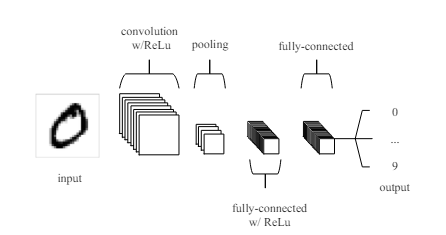
\includegraphics[width=1\linewidth]{CNN.png}
    \caption{A Simple Architecture of CNNs~\cite{o2015introduction}}
    \label{fig:enter-label}
\end{figure}
\begin{figure}[H]
    \centering
    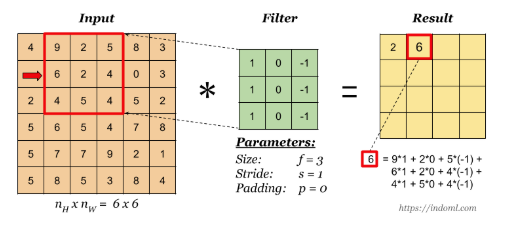
\includegraphics[width=1\linewidth]{Feature Map.png}
    \caption{Process of Applying Filter on Input Image and the Results onto Feature Map\cite{tammina2019transfer}}
    \label{fig:feature map}
\end{figure}
\subsection{Long Short-Term Memory (LSTM)}
The LSTM is an advanced Recurrent Neural Network (RNN) that can solve RNN's vanishing/exploding gradient problem. The LSTM network's memory cell contains three different gates: the input gate, the forget gate, and the output gate. The input gate determines what information we should store in the memory cell, while the forget gate chooses which information to remove from the memory cell \cite{van2020review}. The role of the forget gate is to manage and control what is output from the memory cell.
\begin{figure}[H]
    \centering
    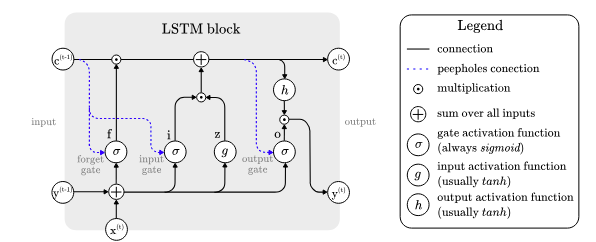
\includegraphics[width=1\linewidth]{Figures/LSTM.png}
    \caption{Architecture of a LSTM block \cite{van2020review}}
    \label{fig:LSTM}
\end{figure}

\subsection{Bidirectional LSTM}
 The BiLSTM model leverages complete sequential information by considering both past and future data points for each position in the sequence, thereby enhancing the original LSTM designed for sequence learning\cite{zhang2017multi}. BiLSTM consists of two LSTMs, and both of them return a probability vector. Their combination forms the final output. This ability of BiLSTMs to process in both directions is especially useful for intricate sequence prediction tasks like examining speech and text.
 \begin{figure}[H]
    \centering
    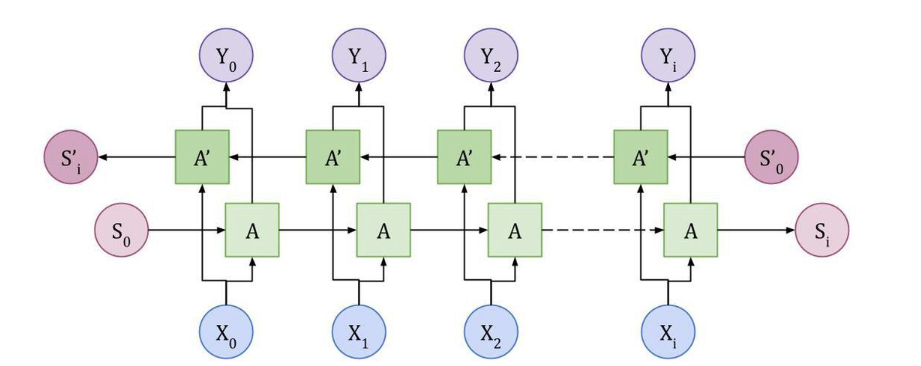
\includegraphics[width=1\linewidth]{image.png}
    \caption{Architecture of a BiLSTM block \cite{bidirectionallstminnlp}}
    \label{fig:BiLSTM}
\end{figure}
Figure \ref{fig:BiLSTM} describes the architecture of the BiLSTM layer where $X_{i}$ is the input, $Y_{i}$ is the output, and A and A' are LSTM nodes~\cite{bidirectionallstminnlp}. The final output of $Y_{i}$ combines A and A' LSTM nodes.

\subsection{Residual Network 50 (ResNet50)}
 ResNet50 is a convolutional neural network (CNN) with 50 layers. ResNet50 is useful for complex tasks involving processing and analyzing images. It contains 48 convolution layers, one MaxPooling layer, and one AveragePooling layer. The main idea behind the ResNet50 model is its unique design using residual blocks. These residual blocks help to solve the vanishing gradient problem. The blocks with residuals have "skip" connections. This lets layers learn residual mappings, which means the network can understand these mappings instead of just direct feature mappings~\cite{he2016deep}. This way of building makes it possible to create deeper networks without losing performance and helps improve the flow of gradients during training, making learning more efficient and stable. This proven CNN is especially useful for feature extraction in complex datasets, including audio spectrograms.
 
\begin{figure}[H]
    \centering
    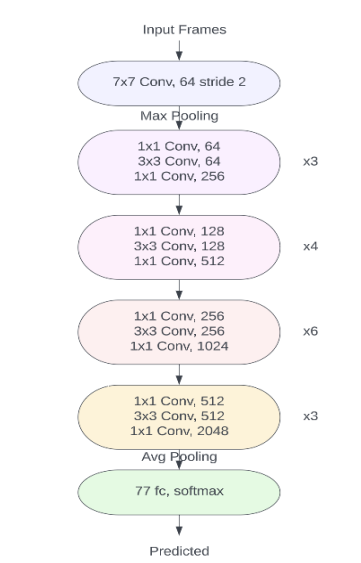
\includegraphics[width=0.5\linewidth]{RetNes50.png}
    \caption{Architecture of a RetNes50~\cite{sehrawat2023deception}}
    \label{fig:ResNet50}
\end{figure}
\subsection{Late Fusion}
We applied a late fusion method, combining audio and text data characteristics. Basically, every type of data has a unique neural network architecture. The results from both models are combined into one vector after being processed separately. Afterward, this combined vector goes into a fusion layer. This layer is where the weights that can be trained are used to find the best weight for each model. The weights have a softmax function applied to them. Softmax will force all outputs to sum up to one. The output of this layer is then processed by a last dense layer with sigmoid activation. Each output provides a probability score showing the possibility of deception. This method, called late fusion, makes our model flexible and adjustable; it learns which features from every data type are more telling about deceitful behavior. 
\begin{figure}[H]
    \centering
    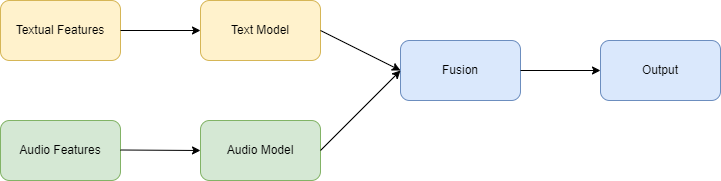
\includegraphics[width=1\linewidth]{High Level Late fusion .drawio.png}
    \caption{A High Level of Late Fusion Model }
    \label{fig:latefusion}
\end{figure}

\subsection{Additional Pretrained Models}
The models mentioned in previous sections have been the focal point of this research. We have spent time fine-tuning them. In addition to those models, we also applied other pre-trained models for comparative analysis. This section will give a brief introduction to each one.
\subsubsection{Bidirectional Encoder Representations from
Transformers (BERT)}
BERT is a language model developed by Google that understands the context of words in a sentence by considering both the words before and after~\cite{devlin2018bert}. It uses a bidirectional approach and a transformer architecture to create context-aware word representations, enabling it to perform well in various natural language processing tasks~\cite{devlin2018bert}.
\subsubsection{Pretrained GPT-2}
 The pretrained GPT-2 model is an advanced language model created by OpenAI that has already learned and been trained on a large amount of text data. This enables it to generate coherent and contextually relevant text based on a given prompt~\cite{solaiman2019release}.
\subsubsection{Pretrained Roberta}
The pretrained RoBERTa (Robustly optimized BERT approach) model, developed by Facebook AI Research, is an improved version of BERT. It enhances performance by optimizing the pretraining process through hyperparameter adjustment, training data modification, and removal of the next sentence prediction task~\cite{liu2019roberta}.
\subsubsection{Pretrained VGG-16}
VGG-16 is a type of CNN consisting of 21 layers in total, but only 16 weight layers. Specifically, VGG-16 has 13 convolutional layers, 5 Max Pooling layers, and 3 fully connected layers. The key feature of VGG16 is its focus on using 3x3 convolution layers with a stride of 1, consistent padding, and a 2x2 maxpool layer with a stride of 2, rather than having numerous hyper-parameters. VGG-16 architecture is shown in Fig \ref{fig:VGG}.
\begin{figure}[H]
    \centering
    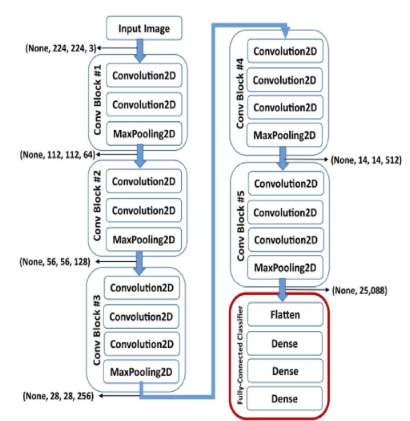
\includegraphics[width=0.8\linewidth]{VGG16.png}
    \caption{The Architecture of VGG-16\cite{theckedath2020detecting}}
    \label{fig:VGG}
\end{figure}
%--------------------------------------------------------------------------------------------------


\section{Experimental Setup}
\label{sec:experimentalsetup}


\subsection{Dataset Description}
\label{sec:dataset}

The Real Life Trial dataset~\cite{csen2020multimodal} has been made by collecting videos from public court trials by Dr. Mihalcea's group at the University of Michigan. It contains a total of 121 brief videos. These videos are divided into 61 videos that depict real instances of deception and 60 videos that depict real instances of truthfulness. In addition to the videos, the dataset also includes transcriptions of each video and annotations of the gestures, such as smile, laugh, scowl, etc, made by the individuals in the videos.


\begin{table}[H]
    \centering
    \begin{tabular}{|p{8cm} p{8cm}|}
        \hline
        \multicolumn{1}{|c}{\textbf{Deceptive}} & \multicolumn{1}{c|}{\textbf{Truthful}} \\
        \hline
        % Insert content for each row here
And he told me that, ammm … he was trying to figure some stuff out, and ammm … I asked him Like what? and he will … I mean I will never forget it, he was smoking a cigarette, and he was like really calm, and he looked at me and he said What would you say if I said … if I told you Laura was dead? And I was like, you know, I was like What? And … basically he told me that, ammm … the night that Laura had come over to the house, that she had died, and that whenever I left that he just panicked and freaked out, and I got … I started freaking out, and I was asking him why he didn't call the cops [stutters] … call for help like he told me he was going to, and he told me that, ammm … he got scared that he was a black man with a dead white woman and nobody was gonna believe him that it was an accident & I have no idea. A police officer I presume. You'd have to ask my mother or my brother. Nope. They said they didn't know where he was being taken. Yep. Went to the house, I was in a fairly catatonic state, my dad and my brother started making phone calls to all the local hospitals, and they eventually got a hold of... I don't know, whatever the hospital is, Atlanta Medical Center. And they wouldn't tell my dad anything but that he was being taken there. So we got in the car, and we left. That's correct. Yes, he was and I had, I -- that was instructed that that was the best idea was to keep him at the day care. The, uh ... Donna. The woman that runs the day care. Yep. That's the safest place ... uh for him to be. \\
        
        \hline
    \end{tabular}
    \caption{Example of Deceptive and Truthful Content}
\end{table}
%-----------------------------------------------------------------------------------------------
\subsection{Preprocessing and Cleaning}
\label{sec:pre}
\subsubsection{Textual data}
Our text processing pipeline involved several steps. First, we removed non-alphabetic characters from the text to ensure only alphabetic letters remain. This step is crucial to avoid any noise in the data that could affect the subsequent processing steps. For conventional models, we used these texts to extract new features. For deep models, we further implemented stemming to each word in the text. Stemming is the process of reducing each word to its root form by removing any suffixes. This step helps to reduce the number of unique words in the text, which is useful for subsequent analysis. After the text had been preprocessed, we performed one-hot encoding. This process involves representing each word in the text as a unique integer index, where the vocabulary size is 5000. This allows us to represent the text in an easily digestible format by machine learning algorithms. Finally, we padded the encoded sequences with zeros to ensure they were all the same length (i.e., 221). This step is important because machine learning algorithms require input data to have a fixed shape. By padding the sequences, we ensured they all had the same number of features, which is necessary for the algorithms to function properly. 
\subsubsection{Audio data}
We converted MP4 video files into WAV audio format. However, we couldn't use deep models to train the raw audio directly. Therefore, our approach was to transform the audio into images, Mel spectrograms. A Mel spectrogram, a visual representation of sound that aligns frequencies to the Mel scale (corresponding to human auditory perception), was used. This was achieved by segmenting the audio, performing a Fourier Transform on each segment to identify frequency content, and then applying Mel scale filters to emphasize perceptually important frequencies. Finally, the Mel spectrograms were converted into the RGB color space and resized to a uniform dimension of 224x224 pixels to ensure consistent input size. Examples of deception and truth images are shown in Figure \ref{fig:dep} and \ref{fig:truth}.

\begin{figure}[H]
    \centering
    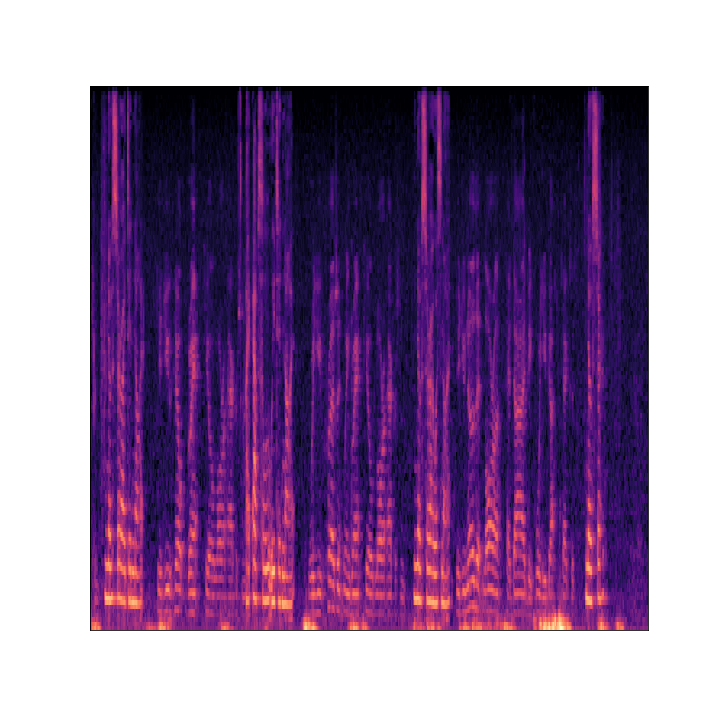
\includegraphics[width=0.5\linewidth]{trial_lie_001.png}
    \caption{Decption Image Example}
    \label{fig:dep}
\end{figure}

\begin{figure}[H]
    \centering
    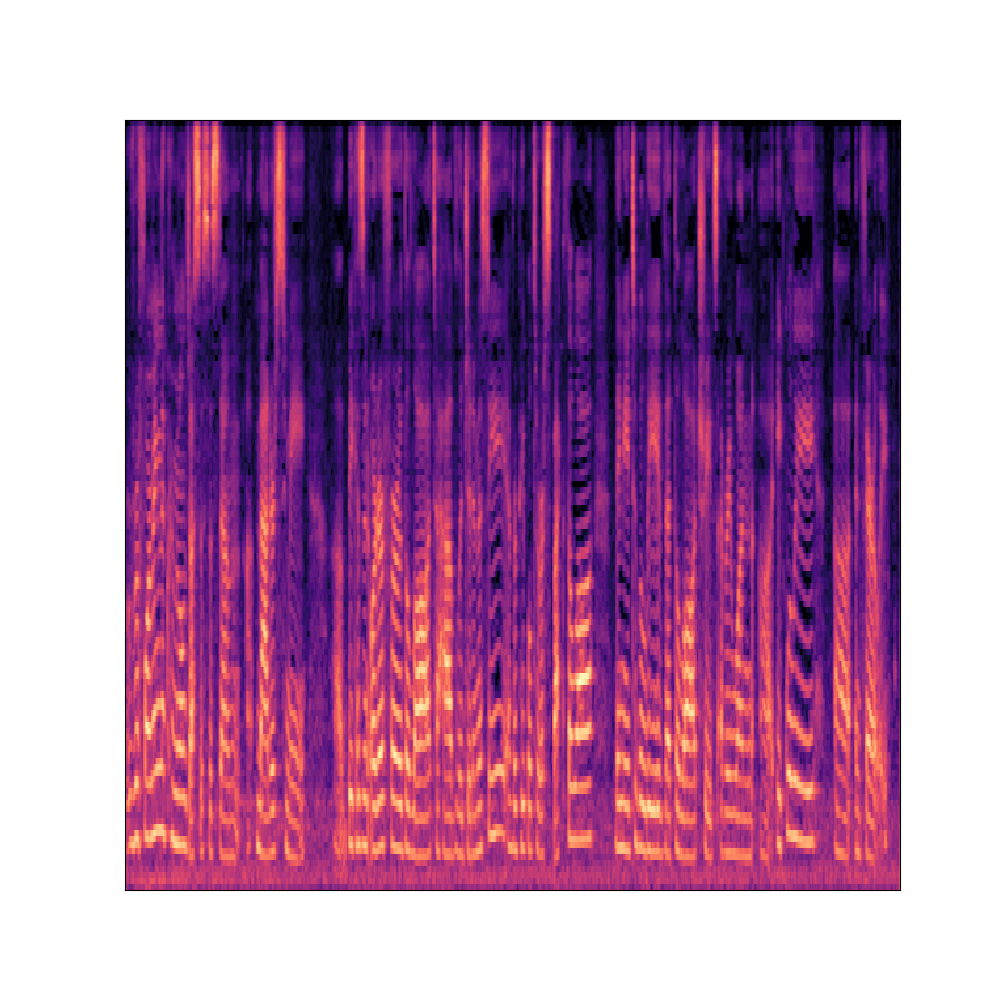
\includegraphics[width=0.5\linewidth]{trial_truth_001.png}
    \caption{Truthful Image Example}
    \label{fig:truth}
\end{figure}
%-----------------------------------------------------------------------------------------------
\subsection{Linguistic Features Extraction}
\label{sec:features}

After preprocessing textual data, we extracted 16 textual features or lexicons that might be considered for lie detection from textual data. For instance, 
the sentiment score in the text is also extracted as a compound score, a measurement that sums up the scores assigned to words in a lexicon, ranging from -1 to 1. A score close to 1 indicates positive emotions, while a score close to -1 indicates negative emotions. A score of 0 represents neutral sentiment. Part-of-speech tagging was used to determine the frequency of adjectives and adverbs, providing insights into the descriptive language used. Additionally, the number of pronouns, conjunctions, and verb tenses (i.e., past, present, future) is computed to understand the speaker's perspective, discourse structure, and temporal references. The count of filler words such as 'um', 'uh', 'hmm' or 'like', repetition of words, negations, and self-references provide further insights into the speaker's fluency, rhetorical style, emphasis, and attempts to persuade the audience. The rest of the features are described in Table II. Together, these features enable a comprehensive text analysis, contributing to lie detection based on linguistic patterns.
\begin{table}[H]
\centering
\begin{tabular}{p{5cm}p{7cm}}
\hline
\textbf{Feature Name} & \textbf{Description} \\
\hline
Word Count & The total number of words in the text. \\
\hline
Sentence Count & The total number of sentences in the text. \\
\hline
Sentiment Score & A numerical score indicating the overall sentiment of the text. \\
\hline
Average Word Length & The average length of words in the text. \\
\hline
Vocabulary Diversity & The ratio of unique words to the total number of words in the text. \\
\hline
Adjective Frequency & The proportion of adjectives in the text. \\
\hline
Adverb Frequency & The proportion of adverbs in the text. \\
\hline
Pronoun Frequency & The proportion of pronouns in the text. \\
\hline
Conjunction Frequency & The proportion of conjunctions in the text. \\
\hline
Past Tense Frequency & The proportion of verbs in the past tense in the text. \\
\hline
Present Tense Frequency & The proportion of verbs in the present tense in the text. \\
\hline
Future Tense Frequency & The proportion of verbs in the future tense in the text. \\
\hline
Filler Word Count & The number of common filler words in the text. \\
\hline
Repetition Count & The proportion of words that appear more than once in the text. \\
\hline
Negation Count & The number of negations in the text. \\
\hline
%Person Entity Frequency & The proportion of words identified as person entities in the text. \\
Self-Reference Count & The number of self-referential words in the text (e.g., "I," "me," "myself"). \\
\hline
    
\end{tabular}
\caption{Description for Extracted Linguistic Features}
\end{table}

\subsection{Model Evaluation}
We evaluated the models using 5-fold cross-validation. The dataset was divided into five subsets, and the training and test sets were created iteratively. During each iteration, one subset was used as the test set, while the remaining four subsets formed the training set. This process was repeated five times, with each subset taking a turn as the test set. This ensures robustness and minimizes overfitting. 
  
The model's performance was evaluated using metrics such as accuracy and the F1 score. 
  
TP: true positives (classifier correct; classifier guessed 1).
  
FP: false positives (classifier incorrect; classifier guessed 1).
  
TN: true negative (classifier correct; classifier guessed 0).
  
FP: false negative (classifier incorrect; classifier guessed 0).
\begin{itemize}
\item Accuracy measures the percentage of correct predictions out of the total instances.
  
  \begin{equation} \label{eq:recall}
    \text{Accuracy} =  \frac{TP + TN}{TP + FP + TN + FN}
\end{equation}
\item The F1 score is the harmonic mean of the precision and recall metrics. Precision measures the percentage of times the classifier was correct when it was predicting the true (1) class. Recall is the percentage of times that the model correctly predicted 1 when the label was, in fact, 1.
  \begin{equation} \label{eq:recall}
    \text{Recall} = \frac{TP}{TP + FN} 
\end{equation}

\begin{equation} \label{eq:recall}
    \text{Precision} = \frac{TP}{TP + FP} 
\end{equation}

\begin{equation} \label{eq:recall}
    \text{F1 score} = \frac{2 * (Precision * Recall)}{Precision + Recall}
\end{equation}

\end{itemize}
%----------------------------------------------


\section{Detection Models}
\label{sec:models}

\subsection{Conventional Models for Textual Data Only}
To train our deception detection models, we explored various conventional algorithms such as:
\begin{enumerate}
    \item Support Vector Machines (SVM) (called Model 1), and
    \item K-Nearest Neighbors (KNN) (called Model 2), and
    \item Logistic Regression (LG) (called Model 3).
    \end{enumerate}

To optimize their performance, we conducted a grid search to fine-tune the hyperparameters of each model. This thorough parameter tuning significantly improved the predictive power of our models. Table \ref{tab:para} listed parameters and their values for the grid search.
\begin{table}[H]
\centering
\begin{tabular}{l c c c}
\hline
\textbf{Model} & \textbf{Parameters}\\
\hline
SVM & \makecell{C: 0.001, 0.1, 1, 10, 100,1000 \\
     kernel: linear, poly, rbf, sigmoid\\
     gamma: scale, auto}\\
\hline
LG & C: 0.001, 0.01, 0.1, 1, 10, 100\\
\hline
KNN &  \makecell{n neighbors : 3, 5, 7 \\
        weights: uniform, distance \\
         p: 1, 2}\\
\hline
\end{tabular}
\caption{Parameter Lists of for Grid Search.}
\label{tab:para}
\end{table}

\subsection{Deep Models and Pre-trained Models for Textual Data Only}
 
\subsubsection{Model 4: 1 BiLSTM}
We created a sequential Bidirectional neural network model. The model had three layers: an embedding layer, a BiLSTM layer, and a dense layer with a sigmoid activation function. The embedding layer mapped the integer-encoded words to dense vectors of fixed size. The BiLSTM layer took the embedded sequence as input and produces a sequence of output vectors. The dense layer outputted a single sigmoid value that represented the probability of the input text being deceptive or truthful. The model was compiled with the binary cross-entropy loss function, the Adam optimizer, and the accuracy metric. 

\subsubsection{Model 5: 1 BiLSTM + Dropout Layer}
 We modified model 5. A dropout layer was added to prevent overfitting, followed by a BiLSTM layer. The output of the LSTM layer was then passed through a GlobalMaxPool1D layer, which selected the maximum value from each feature map, producing a 1D vector. This vector was then passed through two fully connected layers with 64 and 1 neuron(s), respectively, using ReLU and sigmoid activation functions. Finally, the binary cross-entropy loss function optimized the model parameters with the Adam optimizer.
 
\subsubsection{Model 6: 1 BiLSTM + Early Stopping}
 Early Stopping was used to prevent overfitting. The training process stopped if there was no improvement in validation loss for five consecutive epochs.
 
 
 
\subsubsection{Model 7: Bert + Early Stopping + Dropout}
 TFBertForSequenceClassification, a TensorFlow 2.0 compatible implementation of the BERT model for sequence classification, was used. It takes a sequence of tokens as input and outputs a probability distribution over a set of labels for that sequence. It also loaded the pre-trained weights for the specified model, 'bert-base-uncased,' which was a pre-trained BERT model with uncased English text. The loss function used was Sparse Categorical Cross-entropy, which was suitable for multi-class classification tasks. The optimizer was Adam, with a learning rate of 2e-5 and an epsilon value of 1e-08. The model was compiled with the specified loss function, optimizer, and metrics.

\subsubsection{Model 8: Pretrained GPT-2 model}
We built a GPT2 model that was initialized with pre-trained weights using the GPT2Model.from$\_$pretrained() method. A linear layer (i.e., self.fc1) was added to the model that took the hidden states and performed a linear transformation to perform sequence classification. In the $forward()$ method, the input ID and mask were passed to the GPT-2 model, and the output was flattened using $gpt_out.view(batch size,-1)$ and passed through the linear layer to generate the final output. This architecture uses the GPT-2 model as a feature extractor and transforms the extracted features into class predictions.

\subsubsection{Model 9: Pretrained Roberta model}
We built a RoBERTa model for sequence classification using the PyTorch framework and the Hugging Face Transformers library. The 'roberta-base' pre-trained model and tokenizer were used. The input corpus was tokenized, and the resulting tokenized sequences were then padded to a fixed length to ensure consistent input dimensions. The tokenized sequences and corresponding labels were converted into tensors for efficient processing. An Adam optimizer with a learning rate of 2e-5 was used to train the model, while the loss function employed was the cross-entropy loss.

\subsection{Deep Model for Audio data}
\subsubsection{Model 10: ResNet50 + Dropout}
We have modified the model from its original design to suit binary classification tasks, specifically to distinguish between two types of audio signals. The base ResNet50 model, with weights pre-trained on ImageNet, uses transfer learning to take advantage of features learned from visually rich datasets. We hypothesize that this approach will improve the model's ability to recognize subtle patterns in audio spectrogram data. This data shares similarities with image data due to its time-frequency representation. The model uses the ResNet50 base. Its top layer is removed for customization, adjusting the input shape for the task. The last 20 layers are trainable, while earlier layers keep their ImageNet weights. It includes a Global Average Pooling 2D layer, a 0.5 rate Dropout layer, and Early Stopping to prevent overfitting. A Dense layer with 1024 neurons using ReLU activation learns non-linear combinations of features. The final layer is a Dense layer with a single neuron for binary classification. With a 0.0001 learning rate, the Adam optimizer optimizes for binary cross-entropy loss, ensuring learning and generalization.
\subsubsection{Model 10: VGG-16}
We employed a VGG16 base pre-trained on ImageNet, excluding its top layers. All VGG16 layers were initially non-trainable, except those in the final block. Custom layers were added on top, starting with an Input layer, then passing through a GlobalAveragePooling2D layer, a Dropout layer, and a Dense layer with 1024 units and ReLU activation. The final output layer uses a single Dense layer with sigmoid activation. The model is compiled with an Adam optimizer (learning rate of 0.00001), binary cross-entropy loss, and accuracy as a metric.

\subsection{Late Fusion Model for Audio data and Textual data}
We used the ResNet50 model (model 10) for audio data and the BiLSTM model (model 6) for text data to create a late fusion model. We changed the last layers of both models so they would produce a feature vector with 128 dimensions, making sure that features from different types were represented in the same way. The vectors from each model were put together. It made a combined feature vector with 256 dimensions. A specially created LinearW layer took this vector and worked to balance and mix the features coming from both the audio and text paths. The LinearW layer uses a group of weights that can be adjusted and which get better during training. This lets it give each set of features a certain level of importance based on what it has learned. After this fusion layer's output is ready, it goes through another thick layer with sigmoid activation to develop the ultimate prediction.
\begin{figure}[H]
    \centering
    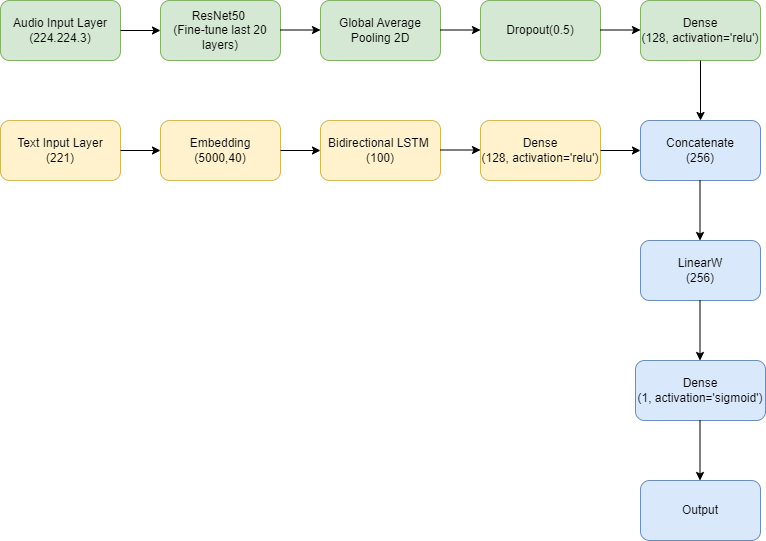
\includegraphics[width=1.1\linewidth]{DetailLateFusion.png}
    \caption{Late Fusion Model for Textual and Audio Data}
    \label{fig:enter-label}
\end{figure}
%--------------------------------------------------------------------------------------------------
\section{Results}
\label{sec:results}

\subsection{Overlapping Probability Density Functions }
PDFs were initially plotted for a selected set of features to understand better the differences in data distribution between the "Lie" and "Truth" categories. These visualizations, displayed as PDFs, offer an intuitive comparison of data distribution shapes. Smoothed PDFs were generated using Kernel Density Estimation (KDE) with a Gaussian kernel. They provided continuous representations of data distributions. These visualizations are useful for identifying features with distinct patterns that could potentially enhance the effectiveness of lie detection based on linguistic analysis.
  
Both PDF plots (Figure \ref{fig:myFig}) and the table (Table \ref{tab:feature-ovl}) visualize and present the quantitative results of the Overlapping Probability Density Functions analysis. This analysis provides a more precise measure of the discriminatory power of individual features in distinguishing between the "Lie" and "Truth" categories. By calculating the OVL scores, we can determine how much the probability density functions of different features overlap between the two categories. 

Features such as "vocabulary diversity" and "conjunction frequency" exhibit high OVL scores. This indicates a substantial overlap in their probability density functions between the "Lie" and "Truth" categories. This suggests that these features may not be strong indicators on their own when it comes to distinguishing between lies and truth. On the other hand, features like "filler word count" and "negation count" display lower OVL scores, implying less overlap in their probability density functions. This indicates a higher potential for effectively distinguishing between "Lie" and "Truth" instances using these features. However, it is important to note that feature interactions and analysis context can significantly influence their discriminatory power.
\begin{figure}[H]
    \begin{subfigure}{0.5\textwidth} % Adjust width for two figures per row
        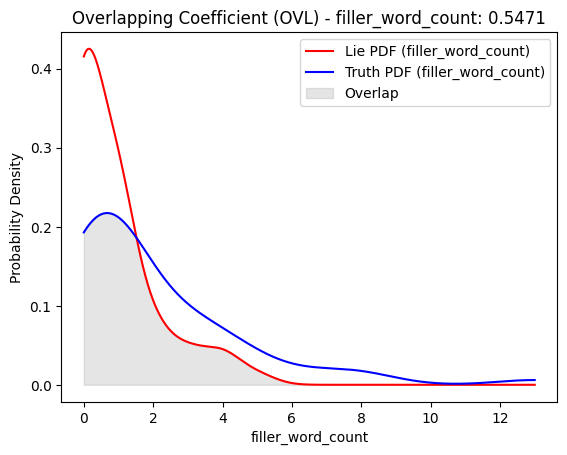
\includegraphics[width=\textwidth]{Figures/filler_word_count.png}
        \caption{PDF for filler word count feature}
        \label{fig:1}
    \end{subfigure}%
    \begin{subfigure}{0.5\textwidth} % Adjust width for two figures per row
        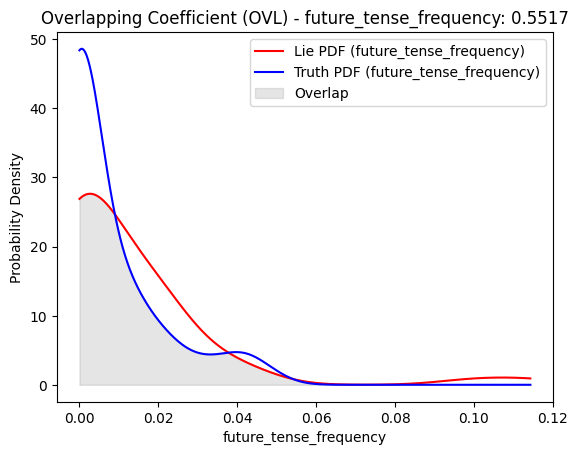
\includegraphics[width=\textwidth]{Figures/future_tense_frequency.png}
        \caption{PDF for future tense frequency feature}
        \label{fig:2}
    \end{subfigure}

    \begin{subfigure}{0.5\textwidth}
        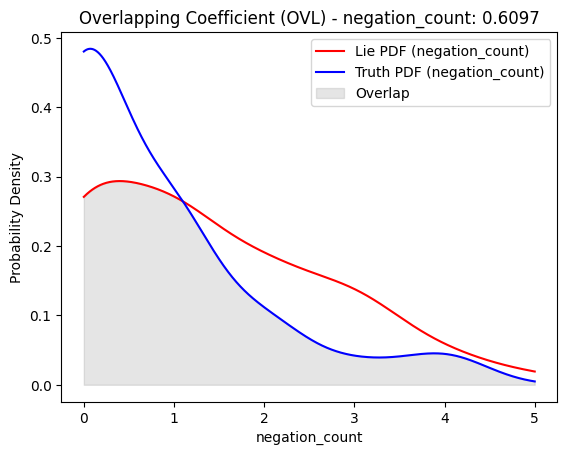
\includegraphics[width=\textwidth]{Figures/negation_count.png}
        \caption{PDF for negation count feature}
        \label{fig:3}
    \end{subfigure}%
    \begin{subfigure}{0.5\textwidth}
        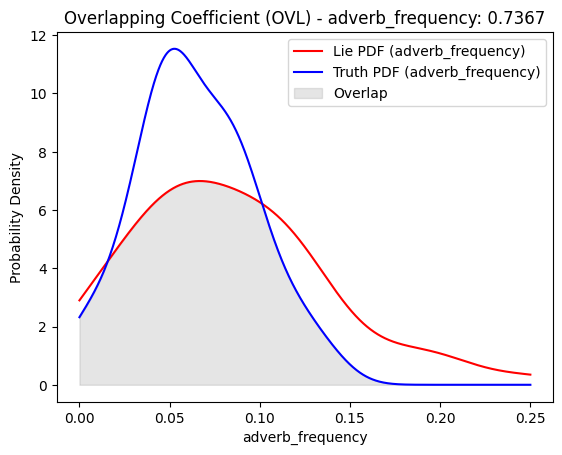
\includegraphics[width=\textwidth]{Figures/adv_frequency.png}
        \caption{PDF for adverb frequency feature}
        \label{fig:4}
    \end{subfigure}

    \begin{subfigure}{0.5\textwidth}
        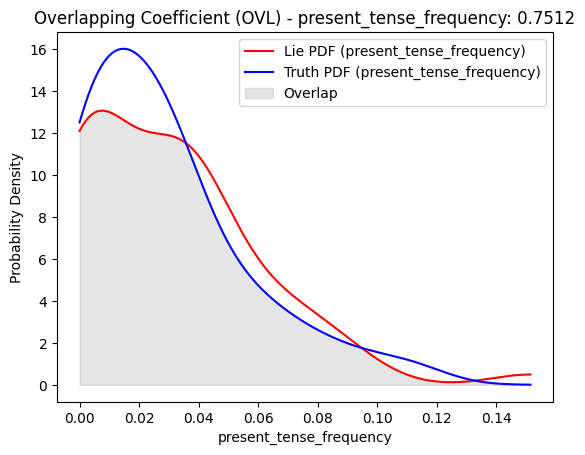
\includegraphics[width=\textwidth]{Figures/present_tense_frequency.png}
        \caption{PDF for present tense frequency feature}
        \label{fig:5}
    \end{subfigure}%
    \begin{subfigure}{0.5\textwidth}
        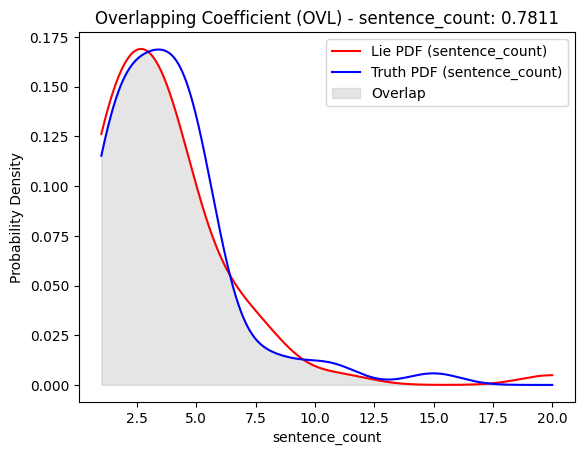
\includegraphics[width=\textwidth]{Figures/sentence_count.png}
        \caption{PDF for sentence count feature}
        \label{fig:6}
    \end{subfigure}
\end{figure}
\begin{figure}
    \ContinuedFloat
    \begin{subfigure}{0.5\textwidth}
        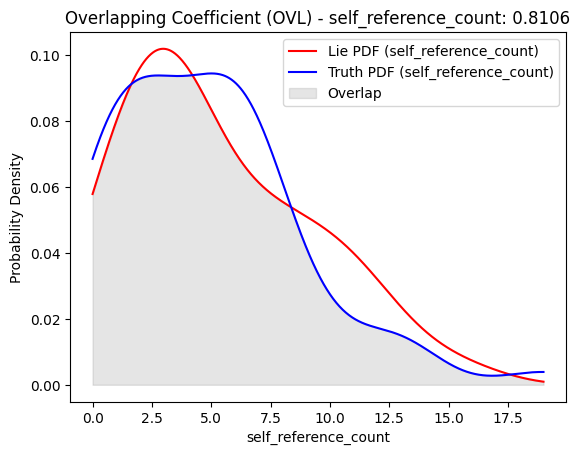
\includegraphics[width=\textwidth]{Figures/self_reference_count.png}
        \caption{PDF for self-reference count feature}
        \label{fig:7}
    \end{subfigure}%
    \begin{subfigure}{0.5\textwidth}
        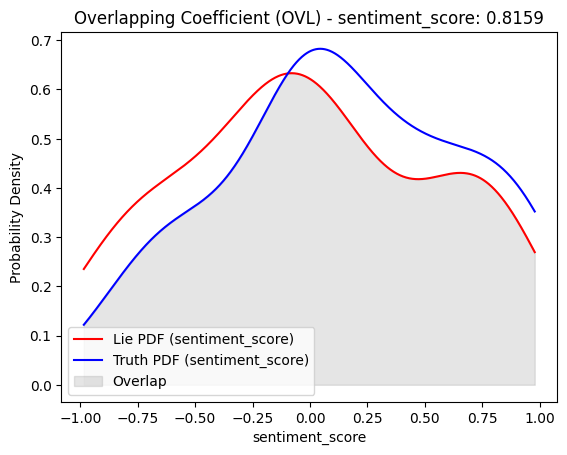
\includegraphics[width=\textwidth]{Figures/sentiment_score.png}
        \caption{PDF for sentiment score feature}
        \label{fig:8}
    \end{subfigure}

    \begin{subfigure}{0.5\textwidth}
        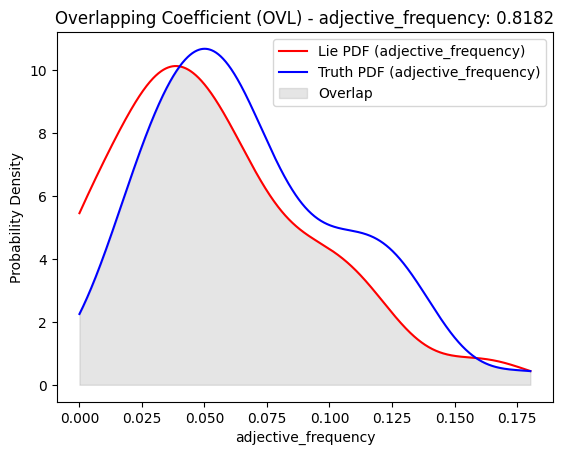
\includegraphics[width=\textwidth]{Figures/adj_frequency.png}
        \caption{PDF for adjective frequency feature}
        \label{fig:9}
    \end{subfigure}
      
    \caption{PDFs for the Top 9 Lowest OVL Scores}
    \label{fig:myFig}
\end{figure}

\begin{table}[H] % Use table* to create a two-column table
\centering
\begin{tabular}{c c}
\hline
\textbf{Features} & \textbf{OVL Score} \\
\hline
filler\_word\_count & 0.5471 \\
future\_tense\_frequency & 0.5517 \\
negation\_count & 0.6097 \\
adverb\_frequency & 0.7367 \\
present\_tense\_frequency & 0.7512\\
sentence\_count & 0.7811 \\
self\_reference\_count & 0.8106 \\
sentiment\_score & 0.8159 \\
adjective\_frequency & 0.8182 \\
word\_count & 0.8214 \\
pronoun\_frequency & 0.8299 \\
past\_tense\_frequency & 0.8345 \\
avg\_word\_length & 0.8479 \\
repetition\_count & 0.8497 \\
conjunction\_frequency & 0.9001 \\
vocabulary\_diversity & 0.9119 \\
\hline
\end{tabular}
\caption{Feature Significance Analysis using OVL}
\label{tab:feature-ovl}
\end{table}

\subsection{Detection Models}
\subsubsection{Conventional Models for Textual Data}
From the initial set of 16 features shown in Table II, OVL, and stepwise feature selection selected different sets of features. For the OVL feature selection approach, we chose the threshold of 0.8, so features with an OVL score less than 0.8 would be selected. Therefore, we had 6 features in total, which were 1) filter work count, 2) future tense frequency, 3) negation count, 4) adverb frequency, 5) present tense frequency, and 6) sentence count. 
In contrast, the stepwise approach carefully chose five features that showed the strongest discriminatory potential: 1) average word length, 2) vocabulary diversity, 3) frequency of adjectives, 4) frequency of adverbs, and 5) the count of filler words. These features played a crucial role in our efforts to detect deception.

 
\begin{table}[H]
\centering
\begin{tabular}{l c c c}
\hline
\textbf{Model} & \textbf{Train Accuracy} & \textbf{Test Accuracy} & \textbf{F1 Score} \\
\hline
Model 1a: SVM + OVL & 61.12 & 59.37 & 70.44 \\
Model 1b: SVM + Stepwise & 64.46 & 63.77 & 69.8 \\
Model 2a: KNN + OVL & 70.65 & 63.6 & 65.47 \\
Model 2b: KNN + Stepwise & 71.69 & 62.83 & 63.07 \\
Model 3a: LR  + OVL & 66.12 & 63.63 & 67.89 \\
Model 3b: LR  + Stepwise & 66.11 & 68.53 & 71.69 \\
\hline
\end{tabular}
\caption{Accuracy and F1 Scores of Conventional Models for Textual Data Only.}
\label{tab:ResultCon}
\end{table}


Table \ref{tab:ResultCon} presents an evaluation of conventional models for both OVL and stepwise feature selection approach in terms of accuracy and F1 scores. Among the three convention models with the OVL approach, SVM (Model 1a) had the lowest test accuracy but the highest F1 score. SVM (Model 1b) achieved relatively lower test accuracy and F1 score for the stepwise approach. KNN (Model 2b) showed reasonable training accuracy but faced challenges in generalization, with a lower test accuracy and F1 score. Among the three different models evaluated, LR (Model 3b) stood out with its test accuracy of 68.53$\%$ and F1 score of 71.69$\%$. These results highlighted the strong potential of this model in distinguishing deceptive actions.

\subsubsection{Deep Models for Textual Data}
Table \ref{tab:ResultDepp} summarizes the performance of different deep models with various architectures and techniques. Model 4, with only one BiLSTM layer, showed improvements in accuracy (67.73$\%$) and F1 score (69.83$\%$), indicating the importance of simplifying the model structure. Model 5 incorporated a Dropout layer alongside a single BiLSTM layer, demonstrating the impact of regularization techniques. However, its accuracy (66.9$\%$) and F1 score (66.18$\%$) were slightly lower than Model 5. Model 6 introduced Early Stopping and significantly enhanced the predictive performance. Model 6 achieved an impressive accuracy of 93.57$\%$ and an F1 score of 94.48$\%$. This finding highlights the importance of monitoring the validation loss during training to prevent overfitting.  Among the three pre-trained models, Model 9 applied pretrained Roberta, giving the highest scores. Table \ref{tab:myTab1} reveals the performance variations among different models and emphasizes the importance of carefully selecting architecture and techniques. The findings further show that regularization techniques, such as Early Stopping, can help prevent overfitting and improve generalization capabilities.
\begin{table}[H]
\centering
\begin{tabular}{l c c c}
\hline
\textbf{Model} & \textbf{Train Accuracy} & \textbf{Test Accuracy} & \textbf{F1 Score} \\
\hline
Model 4:  1 BiLSTM & 100 &  67.73 & 69.83 \\ 
Model 5:  1 BiLSTM + Dropout & 100 & 66.9 & 66.18 \\ 
Model 6: 1 BiLSTM + Early Stopping & 100 &  93.57 &  94.48 \\ 
Model 7: Bert + Early Stopping + Dropout & 83.54&  68.73 & 64.63 \\ 
Model 8: Pretrained GPT2 model & 99.79 &  58.73 & 60.12 \\
Model 9: Pretrained Roberta model & 88.18&  71.2 & 73.71 \\ 
\hline
\end{tabular}
\caption{Accuracy and F1 Scores of Deep Models for Textual Data Only.}
\label{tab:ResultDepp}
\end{table}

\subsubsection{Deep Models for Audio Data}
Table \ref{tab:ResultAudio} shows the performances of audio models. Model 10, which employed the ResNet50 structure, got good training and test accuracy results with 96.04$\%$ and 95.57$\%$, respectively. It also achieved an F1 score of 92.17$\%$. It showed it can generalize well when finding lies in audio. However, Model 11 with VGG16 structure also had good accuracy in training at 96.01$\%$ but a slight drop in test accuracy to 87.63$\%$, and an F1 score of 89.25$\%$. This decrease might show that even though VGG16 is very good for pulling out features, it could be worse at making these features more general than ResNet50.
\begin{table}[H]
\centering
\begin{tabular}{l c c c}
\hline
\textbf{Model} & \textbf{Train Accuracy} & \textbf{Test Accuracy} & \textbf{F1 Score} \\
\hline
Model 10: ResNet50 & 96.04 &  93.57 & 92.16 \\
Model 11: VGG16  & 96.01 &  87.63 & 89.25 \\
\hline
\end{tabular}
\caption{Accuracy and F1 scores of Deep Models for Audio data Only.}
\label{tab:ResultAudio}
\end{table}

\subsubsection{Late Fusion Models for both Textual and Audio Data}
Table \ref{tab:myTab3}  presents how our late fusion model did on five cross-validation folds. On average, this late fusion model got a test accuracy of 90.9$\%$ and an F1 score of 91.07$\%$. The second fold showed the best results for test accuracy and F1 score, with both around 96$\%$.  On the other hand, performance was not as good in the fifth fold; it had an accuracy of about 79.12$\%$ and an F1 score near 82.76$\%$. 
\begin{table}[H]
\centering
\begin{tabular}{c c c c c}
\hline
\textbf{Fold} & \textbf{Audio Weight}  & \textbf{Text Weight} & \textbf{Test Accuracy} & \textbf{F1 Score} \\
\hline
1 & 0.49731752  & 0.50268245 & 92 & 90.9 \\
2 & 0.5032117  & 0.49678826 & 95.83 & 96 \\
3 & 0.516298   & 0.4837021  & 91.67 & 88.89 \\
4&  0.5161787  & 0.48382124 & 95.83 & 96.77 \\ 
5& 0.49938968 &  0.5006103 & 79.12 & 82.76 \\ 
\hline
Average& 0.5064791 & 0.4935209 & 90.9 & 91.07 \\ 
\hline
\end{tabular}
\caption{Weights and Performance Metrics of the Late Fusion Model Across 5 Folds Cross Validation}
\label{tab:myTab3}
\end{table}
%----------------------------------------------------------------------------------------------------------
\section{Discussion}
\subsection{Textual Models}
\subsubsection{Conventional Models}
Average word length, vocabulary diversity, frequency of adjectives, frequency of adverbs, and the count of filler words were selected by stepwise method. On the other hand, the OVL method prioritized a different set of features: the count of filler words, frequency of adverbs, future tense frequency, negation count, and present tense frequency. The OVL approach emphasized features related to grammatical and syntactical aspects, such as tense and negation. These features could provide valuable insights into deceptive language patterns. The count of filler words appeared in both sets of selected features. These words were often used as hesitations or distractions and may serve as markers of deceptive speech. The frequency of the adverbs feature was also included in both selections, suggesting that the intensity or manner of expression in speech could play a role in deception detection.
  
For conventional models using the OVL feature selection method, SVM (Model 1a) delivered the highest F1 score at 70.44$\%$. In contrast, when using features from the stepwise method, LG (Model 3b) achieved the best F1 score. This suggests that the performance of models can vary based on the selected features. LG (Model 3b) attained the highest test accuracy and F1 score among all conventional models with both feature selection methods. However, LR (model 3b) also showed signs of underfitting in our analysis. The relatively low train accuracy of 66.11$\%$ implied that the model struggled to fit the training data adequately. However, the test accuracy is even higher at 68.53$\%$. This difference between train and test accuracy is a classic indicator of underfitting. This underfitting issue may be attributed to the simplicity of the LR model, which may not be able to capture complex, nonlinear relationships within the data. Consequently, the LR model's limited capacity to capture these complex patterns ultimately compromises its overall performance and prevents it from achieving higher accuracy on both the train and test sets. By exploring more sophisticated models, such as deep models, we could strive to improve our models' accuracy and generalization capabilities, ultimately enhancing our analysis's overall performance.

Sen et al.~\cite{csen2020multimodal} also conducted a study where they implemented conventional classifiers such as SVM and RF. They claimed their RF model achieved the highest accuracy of 64.41$\%$ using the Linguistic Inquiry and Word Count (LIWC) lexicon. When comparing it to our conventional model, our LG model (Model 3b) used a smaller feature set and outperformed their RF model in terms of accuracy. This indicates that our feature selection approach played a crucial role in enhancing models' performance by eliminating noise and irrelevant data.

\subsubsection{Deep Models}

We examined regularization techniques and abilities to manage overfitting for the deep models. Model 4, with just 1 BiLSTM layer, showed signs of overfitting. This means it may not perform well on new data. In the context of deep learning model optimization, Dropout and Early Stopping are crucial techniques that play a vital role in addressing the challenges of overfitting and enhancing the overall performance of a model. Dropout is a probabilistic method that helps trim the neural network by randomly dropping out certain units during training, thus achieving a well-balanced distribution of network weights~\cite{sitaula2017analysis}. However, in our case, adding Dropout to Model 5 did not lead to better performance compared to Model 4. Model 5 had similar training accuracy to Model 4 but slightly lower test accuracy and F1 score. This implied that introducing Dropout in Model 5 did not effectively address overfitting or enhance the model's ability to generalize to the test data. Model 6, an extension of Model 4 with the addition of early stopping, showed a significant performance improvement compared to Models 4 and 5. With a test accuracy of 93.57$\%$ and an impressive F1 score of 94.48$\%$, this model balanced precision and recall. It is particularly suitable for tasks where minimizing false positives and false negatives is crucial. While maintaining the high training accuracy observed in Model 4, Model 6 achieved significantly higher test accuracy and F1 score due to the inclusion of early stopping. This indicated that early stopping effectively addressed the overfitting issue in Model 4. Early Stopping is a technique that controls the number of epochs used in both the backpropagation and forward propagation operations, aiming to prevent overfitting and find the optimal point of model performance~\cite{sitaula2017analysis}. These findings emphasized the significance of selecting appropriate regularization techniques to address overfitting and achieve optimal model performance in specific tasks. The success of Model 6 highlighted the importance of early stopping as a powerful tool in deep learning and made it a great choice for applications that value simplicity and high performance. Compared to the BiLSTM-based models, the pre-trained models were not the best choice for the specific task. The effectiveness of a model, whether retrained or not, depends heavily on the dataset's nature and the task's characteristics. 
\subsection{Audio Models}
After looking at the study by Sehrawat et al. on finding deception with CNNs, we realized that when comparing ResNet50 and VGG16 structures, ResNet50 did a better job working with audio data ~\cite{sehrawat2023deception}. Our experimental findings matched this result, showing the ResNet50 model worked better than the VGG16. Another reason why we chose ResNet50 instead of VGG16 was because it took much less time to train, around 8 hours shorter. These findings implied that the ResNet50 model outperformed the VGG16 model in terms of accuracy and computational efficiency. Therefore, we decided to use the ResNet50 architecture in our late fusion model. 
\begin{table}[H]
\centering
\begin{tabular}{l c c}
\hline
\textbf{Model} & \textbf{Test Accuracy} & \textbf{F1 Score} \\
\hline
Model 12: Late Fusion Model & 90.9 & 91.07 \\
Sehrawat et al.~\cite{sehrawat2023deception}& 80 & xxx\\
Zhang et al.~\cite{zhang2022fine} & 84.40 & 70.80  \\
\hline
\end{tabular}
\caption{Comparison of Test Accuracy and F1 Scores for Our Late Fusion Model Against Previous Work}
\label{tab:myTab4}
\end{table}
  
\subsection{Late Fusion Model}  
Table \ref{tab:myTab4} shows our late fusion model outperforms the recent previous model in both test accuracy and F1 scores. With 90.9$\%$  in accuracy and an F1 number of 91.0$\%$, our model did much better compared to Sehrawat et al.'s method with 80$\%$  accuracy and Zhang et al. 's work that had a correct rate of 84.40$\%$. Our model performed much better, especially in the F1 score, which exceeded Zhang et al. 's 70.80$\%$  by more than 20 percent points. This big difference highlighted how well our design worked because it cleverly used both audio and textual data to get better at spotting deception.  

We saw a consistent balance between audio and text inputs when we looked carefully at how the last layer of fusion gives out weights over five validation folds. There was only a small change around an almost equal division. This showed that our model was strong because even little changes in the weights, which went from about 49.7$\%$ to 51.6$\%$ for audio and then similar for text, were good enough to handle the slight differences in each fold's information. The balance that was always the same made sure one way of getting information did not take over so the model could use what was good about both audio and textual data. This careful way of deciding importance really helped make the model work very well and be trusted with different kinds of information because it mixed ways to get knowledge together in a smart way to find deception.
%----------------------------------------------------------------------------------------------------------
\section{Conclusion and Future Work}
\label{sec:conclusion}
In this work, we extracted a total of 16 textual features. Using both the stepwise method and the OVL method, we identified 5 highly significant features from each approach. We conducted experiments using both conventional models and deep models. Our findings showed that LR achieved the highest accuracy among the conventional models with an impressive 68.53$\%$ and an F1 score of 71.69$\%$. However, the deep model, which consisted of a single layer of BiLSTM with Early Stopping, outperformed all other textual models. This deep model achieved an outstanding accuracy of 93.57$\%$ and an F1 score of 94.48$\%$. 
  
For audio data, our ResNet50 model achieved an accuracy of 93.57$\%$ and an F1 score of 92.16$\%$. In a further comprehensive approach using both textual data and audio data, we accomplished an accuracy of 90.9$\%$ and an F1 score of 91.07$\%$, which outperformed other text and audio models from previous research.

In this work, we created textual models and audio models. For future work, we plan to extract new features from video. We will develop new and improved detection models by combining video features with audio features and the textual features used in this work. Integrating multiple modalities can provide a more comprehensive understanding of the phenomenon under investigation. Besides, it is worth mentioning that the Real Life Trial dataset is relatively small. While the findings from this dataset are promising, experimenting with larger datasets would significantly enhance the robustness and generalizability of our model. We can ensure our findings hold across different contexts and populations.
%----------------------------------------------------------------------------------------------------------
\newpage

\bibliographystyle{IEEEtran}
\bibliography{IEEEfull,sample-base}
%-------------------------------------------------------


%------------------------------------------------------------------------------------------
\clearpage



%------------------------------------------------------------------------------------------


\end{document}
